%%%%%%%%%%%%%%%%%%%%%%%%%%%%%%%%%%%%%%%%%%%%%%%%%%%%%%%%%%%%%%%%%%%%%%%%%%%
%
% Plantilla para un artículo en LaTeX en español.
%
%%%%%%%%%%%%%%%%%%%%%%%%%%%%%%%%%%%%%%%%%%%%%%%%%%%%%%%%%%%%%%%%%%%%%%%%%%%



%--------------------------------------------------------------------------
\title{Plantilla para un artículo \LaTeX}
\author{El autor va aquí\\
  \small Dept. Plantillas y Editores\\
  \small E12345\\
  \small España
}


\begin{document}
\begin{center}
\textbf{PRACTICA DE LABORATORIO N° 01:} \\
\textbf{Elaboración de Dashboards en Power BI} \\
\end{center}

\section{REQUERIMIENTOS}
\textbf{ } \\
\textbf{- Conocimientos} \\
\textbf{✓ Para el desarrollo de esta práctica se requerirá de los siguientes conocimientos básicos:}
\item{- Conocimientos básicos de administración de base de datos Microsoft SQL Server.\\
- Conocimientos básicos de SQL.\\\\
\textbf{- Software} \\
\textbf{✓ Asimismo se necesita los siguientes aplicativos:} \\
- Microsoft SQL Server 2016 o superior\\
- Base de datos AdventureWorks2016 o superior\\
- Power BI Desktop.\\
- Tener una cuenta Microsoft registrada en el Portal de Power Bi}\\

\section{CONSIDERACIONES INICIALES}
\item{Generar una carpeta o directorio Power BI en un lugar accesible para guardar los resultados de la práctica.}
\section{DESARROLLO}
\textbf{Tarea 1: Conectar a SQL Server desde Power BI Desktop} \\
\item{- Cuando la Ventana de Power BI Desktop aparezca, en el panel a mano izquierda, hacer click en Obtener
Datos (Get Data).}
\item{- En el cuadro de dialogo Obtener Datos (Get Data), click en base de datos SQL Server, y luego hacer click en
Conectar (Connect).}
\begin{center}
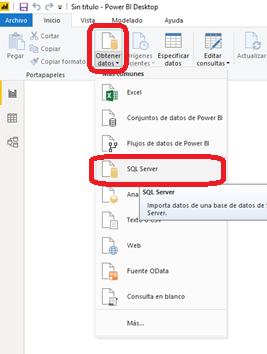
\includegraphics[width=10cm]{./Imagenes/image001}
\end{center}

\item{- En el cuadro de dialogo base de datos SQL Server, en la casilla servidor tipear (local), en la casilla Base de
datos (opcional) / Database (optional), tipear AdventureWorks2017, y hacer clic en OK. }
\begin{center}
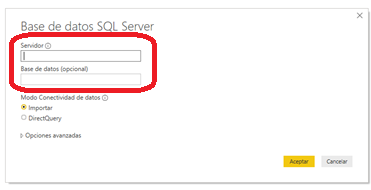
\includegraphics[width=10cm]{./Imagenes/image002}
\end{center}

\newpage
\item{- En el cuadro de dialogo Navegador (Navigator), seleccionar la vista Sales.vStoreWithDemographics después Sales.vStoreWithDemographics, y luego
hacer click en Cargar (Load). }
\begin{center}
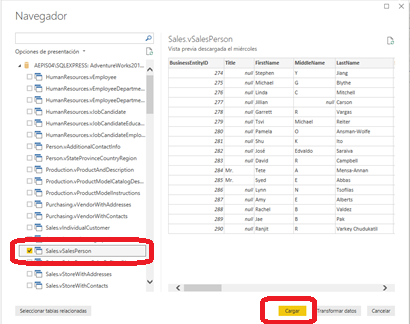
\includegraphics[width=12cm]{./Imagenes/image003}
\end{center}

\item{- En el cuadro dialogo base de datos SQL Server, en la casilla Servidor (Server), tipear (local), y en la casilla
Base de datos (opcional), tipear AdventureWorks2017.}
\item{- Expandir opciones Avanzadas, en la casilla sentencia SQL (opcional, base de datos requerida), tipear la
siguiente consulta, y luego hacer click en OK:}
\begin{center}
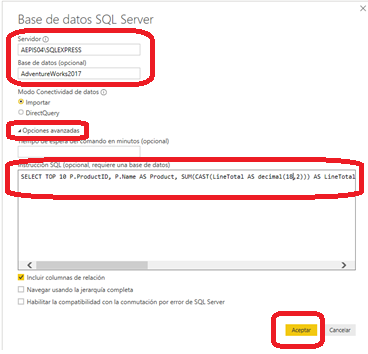
\includegraphics[width=10cm]{./Imagenes/image004}
\end{center}
\begin{center}
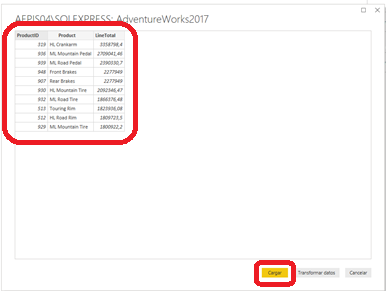
\includegraphics[width=10cm]{./Imagenes/image005}
\end{center}
\textbf{Tarea 2: Adicionar Gráficos al Reporte}
\item{- Al final tendremos los siguientes graficos con los datos obtenidos de la base de datos AdventureWorks2017. }
\begin{center}
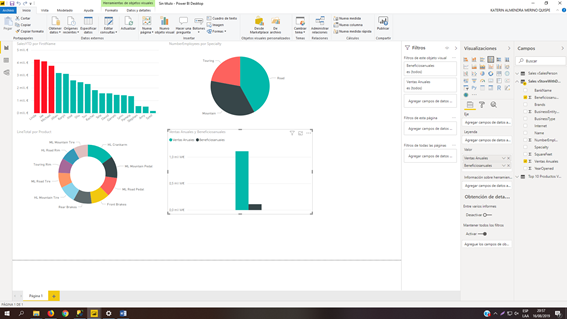
\includegraphics[width=12cm]{./Imagenes/image006}
\end{center}

\newpage
 \item{- En el menu Archivo (File menu), hacer click en Guardar (Save), crear un directorio Power BI, y guardar el archive como Ventas de Adventure Works Sales}
\begin{center}
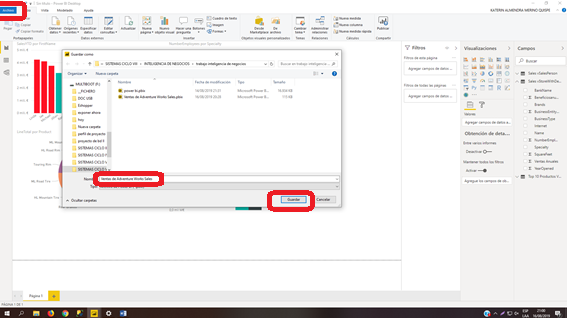
\includegraphics[width=12cm]{./Imagenes/image007}
\end{center}

\textbf{Tarea 3: Publicar el reporte en el portal de Power BI}
\item{Guardamos y Subimos nuestro proyecto a nuestra cuenta de powerbi. }
\begin{center}
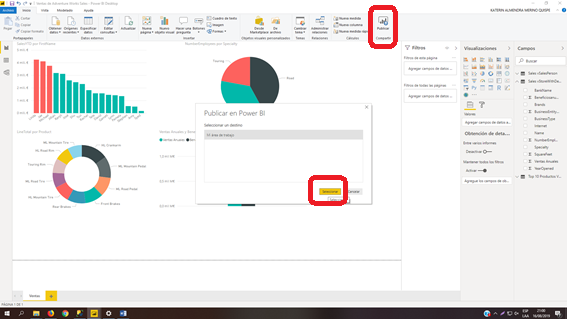
\includegraphics[width=12cm]{./Imagenes/image008}
\end{center}

\item{el link para poder vizulaizar el trabajo encargado numero 1 .\\
https://app.powerbi.com/groups/me/reports/85dd506c-f7e3-40a4-a7cb-58216881d9f6/ReportSection }



\end{document}
